\documentclass[10pt]{scrartcl}
\usepackage{geometry}
\usepackage[parfill]{parskip}
\usepackage{graphicx}
\usepackage{amssymb}
\usepackage{epstopdf}
\usepackage{color}
\usepackage{tikz}
\usetikzlibrary{positioning}
\usetikzlibrary{arrows,automata}

\usepackage{listings}

\lstdefinelanguage{FSharp}%
{morekeywords={let, new, match, with, rec, open, module, namespace, type, of, member, val, %
and, for, while, true, false, in, do, begin, end, fun, function, return, yield, try, %
mutable, if, then, else, cloud, async, static, use, abstract, interface, inherit, finally },
otherkeywords={ let!, return!, do!, yield!, use!, var, from, select, where, order, by },
keywordstyle=\color{bluekeywords},
sensitive=true,
basicstyle=\ttfamily,
breaklines=true,
xleftmargin=\parindent,
aboveskip=\bigskipamount,
tabsize=4,
morecomment=[l][\color{greencomments}]{///},
morecomment=[l][\color{greencomments}]{//},
morecomment=[s][\color{greencomments}]{{(*}{*)}},
morestring=[b]",
showstringspaces=false,
literate={`}{\`}1,
stringstyle=\color{redstrings},
} 

\lstset{
  frame=single,language=FSharp,
   basicstyle=\footnotesize,
  escapechar=\@,
  basicstyle=\footnotesize, frame=tb,
  numbers=left,
  stepnumber=2,
  numbersep=5pt, 
  numberstyle=\tiny\color{mygray},
  xleftmargin=.1\textwidth, xrightmargin=.1\textwidth
}
\usepackage{geometry}
 \geometry{
 a4paper,
 total={210mm,297mm},
 left=20mm,
 right=20mm,
 top=20mm,
 bottom=20mm,
 }
\definecolor{bluekeywords}{rgb}{0.13,0.13,1}
\definecolor{greencomments}{rgb}{0,0.5,0}
\definecolor{redstrings}{rgb}{0.9,0,0}
\definecolor{mygray}{rgb}{0.2,0.2,0.2}

\DeclareGraphicsRule{.tif}{png}{.png}{`convert #1 `dirname #1`/`basename #1 .tif`.png}

\title{02257 - Applied functional programming}
\subtitle{Project 3 - A game with a graphical user interface}
\author{Anna Maria Walach - \textit {s121540@student.dtu.dk} \\ Kim Rostgaard Christensen - \textit {s084283@student.dtu.dk}}
\begin{document}
\maketitle
\section{Type declarations}
The main types used in applications are presented in listing \ref{list:types}. 
\begin{figure} [!ht]
\begin{lstlisting}
type NimPlayer    = AI | Human
type NimGameState = State of List<int>
type NimGame      = Nim of State * NimPlayer
type GameEvent = Move of AsyncEventQueue<GameEvent> * int * int | EndGame of AsyncEventQueue<GameEvent> * NimPlayer | StartGame of AsyncEventQueue<GameEvent> * NimGameState
type NimGameUI = GameUI of List<string> * AsyncEventQueue<GameEvent>

\end{lstlisting}
\caption{Main types used in Nim application}
\label{list:types}
\end{figure}
\section{Signatures of the main functions}
\begin{figure} [!ht]
\begin{lstlisting}
//AI module
val nextMove : State -> State
//GUI module
val updatePanels : Panel -> Panel -> Panel-> Form -> unit ()
val generateButtonMatches : State -> (int -> int -> unit()) -> Control [];;
\end{lstlisting}
\caption{Signatures of main functions from AI and GUI module}
\label{list:types}
\end{figure}
\subsection{NimAI}
This module provide one main function (line 1 in listing \ref{list:types} and three helper function (for 3 difficulty levels), that are not being accessed anywhere beside the module and has exactly the same signatures. 
\subsection{NimGUI}
NimGUI has a lot of interesting functions, but we decided to only pick two most important. The first one (line 3 in listing \ref{list:types} has a side effects - it actually only update properties of elements send to it (it's a refresh function). Second one is one of the few functions that has another function as an argument - a click handler.
\subsection{NimGame}
The type \texttt{NimGameUI} has a factory function \texttt{create} that takes a \texttt{List<int>} as argument and can be used along with the \texttt{window} operation. The \texttt{window} function returns a \texttt{Form} that can be used outside the module in -- for instance -- an argument to the \texttt{Application.Run} function. This is exactly what is done in the \texttt{NimLauncher} for spawning new games. \texttt{NimLauncher} has \texttt{create} and  \texttt{window} operations similar to \texttt{NimGameUI}.

%Something about the button generation function, gameUI, launcher and game object creation and manipulation.

\section{Structure overview}
We've divided the user interface of the game into two larger components; the launcher and the game itself. The launcher handles download of games and may bootstrap the a game user interface with a downloaded game configuration. The launcher builds up a list of known games from a list of urls. These are hardcoded as of now, but could just as well be initialized by a line-separated text file.
\subsection{Modules}
The complete application itself is designed by the \emph{separation of concerns} principle and the following contains 5, largely independent, modules:
\begin{itemize}
  \item \texttt{NimMain} - script that acts as the starting point for the whole application.
  \item \texttt{NimLauncher} - module responsible for handling the logic of download game window and spawning new game windows.
  \item \texttt{NimGame} - module responsible for handling the logic of the game
  \item \texttt{NimGUI} - module, that stores, updates and creates almost all GUI elements for \texttt{NimLauncher} and \texttt{NimGame}.
  \item \texttt{NimAI} - small modules that stores and provide functions to generate the AI move
\end{itemize}

\subsection{Finite automatons}
As we have two major UI components, we also have two automatons in our game. The first one is part of the launcher (automaton below to the left) controls UI behavior and appearance. Once ready, a download click handler in the UI will send the automaton to the \textbf{Loading} State where it can either be cancelled, succeed or return an error. Once the download is done, the automaton will automatically go back to \textbf{Ready}, accepting new fetch commands. The UI responds to the commands by, when downloading, disabling every button -- except for the \textbf{Abort button}. When \textbf{Loading} completes, it will re-enable the buttons and -- if successful -- add a click handler for the launch button correlated with the download button that launches a new game UI instance. 

\begin{center}
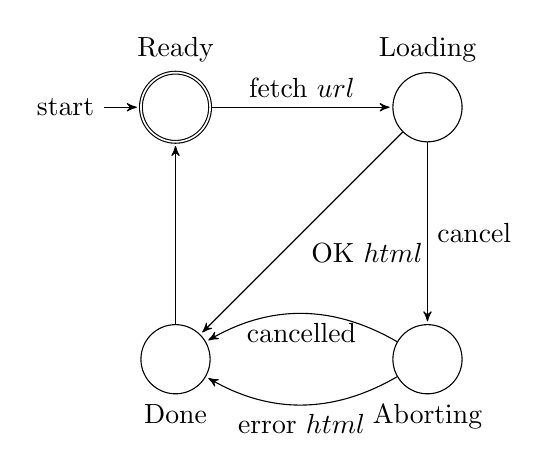
\begin{tikzpicture}[>=stealth',shorten >=1pt,auto,node distance=3.2cm]
  \node[initial,state,accepting,label=above:Ready] (Ready)                       {};
  \node[state,label=above:Loading]                 (Loading)  [right of=Ready]   {};
  \node[state,label=below:Aborting]                (Aborting) [below of=Loading] {};
  \node[state,label=below:Done]                    (Done)     [below of=Ready]   {};

  \path[->]
        (Ready) edge              node {fetch $url$}  (Loading)
      (Loading) edge              node {cancel}       (Aborting)
     (Aborting) edge [bend left]  node {error $html$} (Done)
     (Aborting) edge [bend right] node {cancelled}    (Done)
      (Loading) edge              node {OK $html$}    (Done);
  \path[->,label]
         (Done) edge              node {}             (Ready); 
\end{tikzpicture} \hspace{10mm} 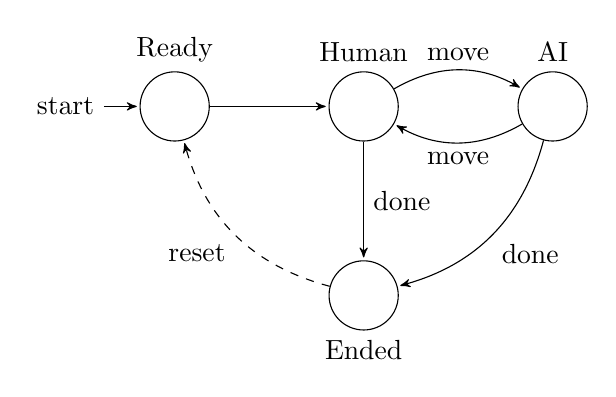
\begin{tikzpicture}[>=stealth',shorten >=1pt,auto,node distance=2.4cm]
  \node[initial,state,label=above:Ready] (Ready)                   {};
  \node[state,label=above:Human]         (Human)  [right of=Ready] {};
  \node[state,label=above:AI]            (AI)     [right of=Human] {};
  \node[state,label=below:Ended]         (Ended)  [below of=Human] {};


  \path[->]
     (Ready)  edge              node {} (Human)
      (Human) edge [bend left]  node {move} (AI)
        (AI)  edge [bend left] node {done} (Ended)
        (AI)  edge [bend left]  node {move} (Human)
      (Human) edge  node {done} (Ended);
  \path[->, dashed]
      (Ended) edge [bend left] node {reset} (Ready); 
\end{tikzpicture}
\end{center}
The automaton for the game logic (above to the right) works by initializing a game object within the \textbf{Ready} state and then alternating it between \textbf{AI} and \textbf{Human} until there are no matches left in any heaps.
The reset signal may, technically speaking, be sent from every state but these transitions have been left out of the diagram to avoid clutter.
The automaton will then go to the \textbf{Ended} state and notify the player whether or not he/she has won or not. After a move (\textbf{AI} or \textbf{Human}), the panel with the matches will re-render, giving the visual representation of the current game. A move is performed by clicking a match. That match will then spawn a move operation stating which index it has and which heap it belongs to. The state machine will then reflect the move to the state and re-render. 

%type Message =
%  | Download of string * Control * Control| Cancel | Web of string | Error | Cancelled 
Note: naming and other minor differences between model and code are present in the current state of the project and should be considered as design models.
\section{Extensions}
There is a possibility to restart an ongoing game and also set the difficulty. There are currently three levels of difficulty implemented; easy, intermediate and hard. They work by adjusting the AI's probability of ''making mistakes`` by performing a random move rather than a strategic one.

You can play multiple rounds of a single game using the game interface, or you have the possibility to close the game UI and return to the launcher to download and start a different game.

We've extended the basic solution with a more accurate graphical representation of the heap and added a cute kitten theme to the interface to give it a humorous touch, which can be seen in the screenshots below. The launcher is to the left, and the game is to the right.
\begin{center}
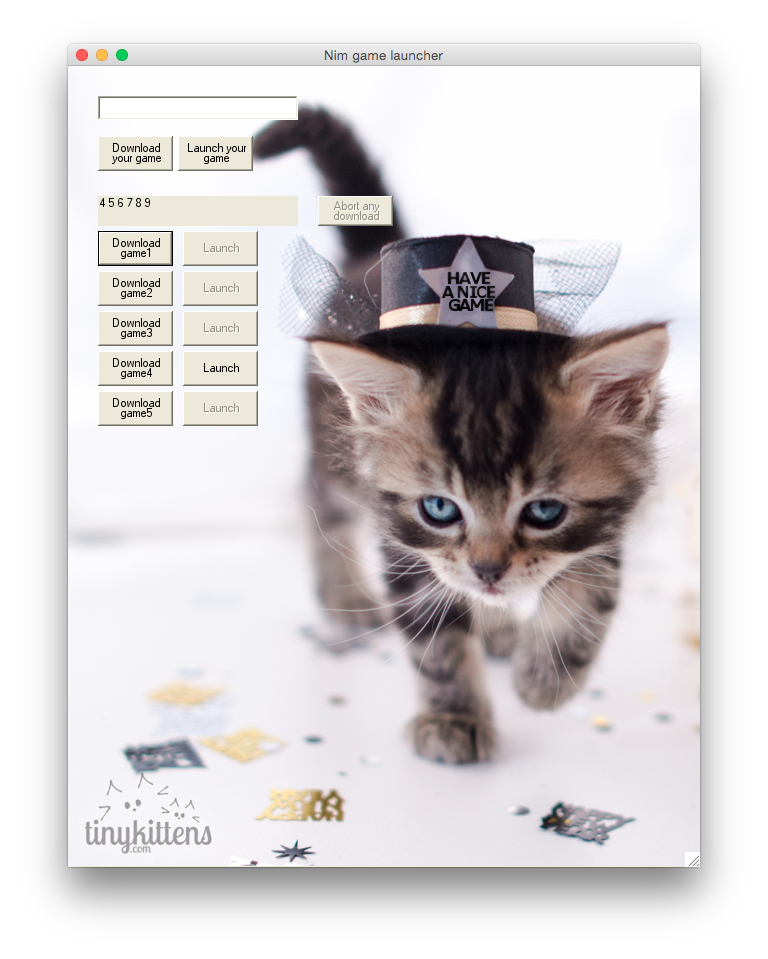
\includegraphics[width=0.49\textwidth]{launcher_ui} 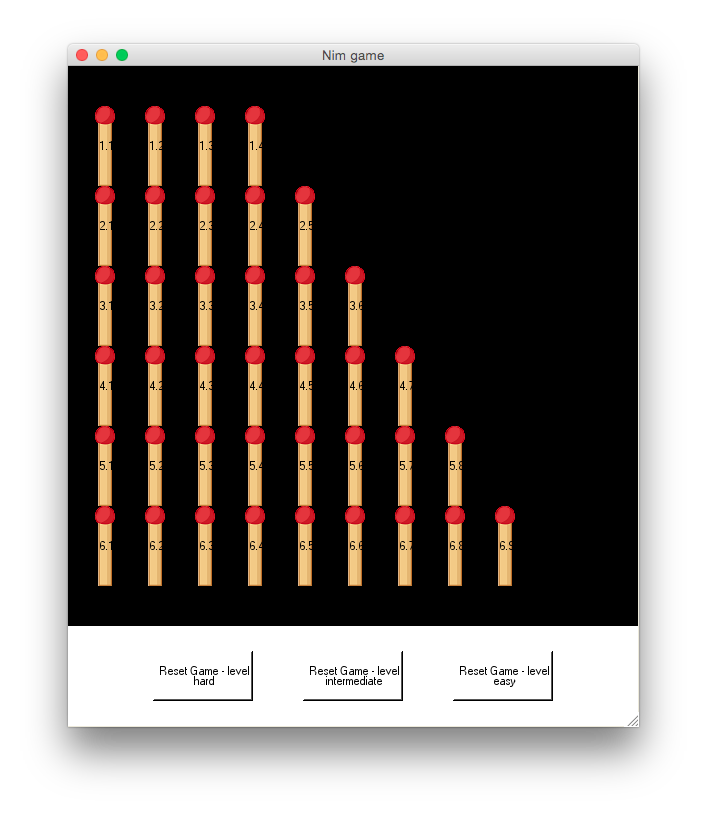
\includegraphics[width=0.49\textwidth]{game_ui}
\end{center}

\section{Conclusions}
The design pattern handed out was found to be very suitable for creating responsive graphical user interfaces, but was challenging to break into reusable modules. MVC is implemented to some extent, but is hard to realize due to lack of multicast support in the \texttt{AsyncEventQueue} which would have made it possible for multiple UI components to, independently, listen for model changes. 
\bibliographystyle{plain}
\bibliography{references}

\end{document}  
